% Created 2018-10-12 Fri 17:55
% Intended LaTeX compiler: pdflatex
\documentclass[conference]{IEEEtran}

\usepackage{graphicx}
\usepackage{amssymb}
\usepackage{amsmath}
\usepackage{colortbl}
\usepackage{xcolor}
\usepackage{url}
\usepackage{listings}
%\usepackage[utf8]{inputenc}
\usepackage[english]{babel}
\usepackage{multirow}
\usepackage{caption}
\usepackage{hyperref}
\usepackage{booktabs}
\usepackage{array}
\usepackage{relsize}
\usepackage{bm}
\usepackage{wasysym}
\usepackage{ragged2e}
\usepackage{todonotes}
\usepackage{tabularx}
\lstset{ %
backgroundcolor={},
basicstyle=\ttfamily\scriptsize,
breakatwhitespace=true,
breaklines=true,
captionpos=n,
extendedchars=true,
frame=n,
rulecolor=\color{black},
showspaces=false,
showstringspaces=false,
showtabs=false,
stepnumber=2,
stringstyle=\color{gray},
tabsize=2,
}
\renewcommand*{\UrlFont}{\ttfamily\smaller\relax}
\makeatletter
\def\maketag@@@#1{\hbox{\m@th\normalfont\normalsize#1}}
\makeatother
\graphicspath{{./img/}}
\renewcommand*{\UrlFont}{\ttfamily\smaller\relax}
\author{\IEEEauthorblockN{Pedro Bruel\IEEEauthorrefmark{1}\IEEEauthorrefmark{2},
Arnaud Legrand\IEEEauthorrefmark{1},
Brice Videau\IEEEauthorrefmark{1},
Jean-Marc Vincent\IEEEauthorrefmark{1}, and
Alfredo Goldman\IEEEauthorrefmark{2}}
\IEEEauthorblockA{\IEEEauthorrefmark{1}University of Grenoble Alpes, CNRS, INRIA, Grenoble INP, LIG -- 38000 Grenoble, France\\
Email: \{arnaud.legrand, brice.videau, jean-marc.vincent\}@imag.fr}
\IEEEauthorblockA{\IEEEauthorrefmark{2}University of São Paulo -- São Paulo, Brazil\\
Email: \{phrb, gold\}@ime.usp.br}}
\date{\today}
\title{Autotuning under Tight Budget Constraints:  \\ A Transparent Design of Experiments Approach}
\hypersetup{
 pdfauthor={},
 pdftitle={Autotuning under Tight Budget Constraints:  \\ A Transparent Design of Experiments Approach},
 pdfkeywords={},
 pdfsubject={},
 pdfcreator={Emacs 26.1 (Org mode 9.1.14)},
 pdflang={English}}
\begin{document}

\maketitle
\begin{abstract}
A large quantity of resources is spent writing, porting, and optimizing
scientific and industrial High Performance Computing applications. Autotuning
techniques have become therefore fundamental to lower the costs of leveraging
the improvements on execution time and power consumption provided by the latest
software and hardware platforms. Yet, most popular autotuning techniques still
require a large budget of costly experimental measurements to provide good
results while rarely providing exploitable knowledge about the problem after
optimization. In this paper we present a user-transparent autotuning technique
based on Design of Experiments that operates under tight budget constraints by
significantly reducing the amount of measurements needed to find good
optimizations. Our approach also enable users to make informed decisions on what
optimizations to pursue and when to stop optimizing. We present experimental
evaluations of our approach and show that, leveraging user decisions, it is
capable of finding the global optimum of a GPU Laplacian kernel optimization
using half of the measurement budget used by other common autotuning techniques.
We also show that our approach is capable of finding speedups of up to
\(50\times\) for some kernels from the SPAPT benchmark using up to \(10\times\) less
measurements than random sampling.
\end{abstract}

\section{Introduction}
\label{sec:orgd92e770}
Optimizing code for objectives such as performance and power consumption is
fundamental to the success and cost effectiveness of industrial and scientific
endeavors in High Performance Computing. A considerable amount of highly
specialized time and effort is spent in porting and optimizing code for GPUs,
FPGAs and other hardware accelerators. Experts are also needed to leverage
bleeding edge software improvements in compilers, languages, libraries and
frameworks. The objective of techniques for the automatic configuration and
optimization of High Performance Computing applications, or \emph{autotuning}, is to
decrease the cost and time needed to adopt efficient hardware and software.
Typical autotuning targets include algorithm selection, source-to-source
transformations and compiler configuration.

Autotuning can be studied as a search problem, where the objective is to
minimize single or multiple software of hardware metrics. The exploration of the
search spaces defined by configurations and optimizations present interesting
challenges to search strategies. These search spaces grow exponentially with the
number of considered configuration parameters and their possible values. They
are also difficult to extensively explore due to the often prohibitive costs of
hardware utilization and program compilation and execution times. Developing
autotuning strategies capable of producing good optimizations while minimizing
resource utilization is therefore essential. The capability of acquiring
knowledge about an optimization problem is also a desired feature of an
autotuning strategy, since this knowledge can decrease the cost of subsequent
optimizations of the same application or for the same hardware.

It is common and usually effective to use search meta-heuristics such as genetic
algorithms and simulated annealing in autotuning. These strategies attempt to
exploit local properties, but are generally incapable of fully exploiting global
search space structures. Seymour \emph{et al.}~\cite{seymour2008comparison} and
Knijnenburg \emph{et al.}~\cite{knijnenburg2003combined} report that these
strategies are not more effective than a naive uniform random sample of the
search space, and usually rely on a large number of measurements and frequent
restarts to achieve good performance improvements. Search strategies based on
gradient descent are also commonly used in autotuning and also rely on a large
number of measurements. Their effectiveness diminishes significantly in search
spaces with complex local structures. Completely automated machine learning
\todo{ref} autotuning strategies are promising in building models for predicting
important optimization parameters, but still rely on a sizable data set for
training. Large data sets are fundamental to strategies based on machine
learning since they select models from a generally very large class.

Search strategies based on meta-heuristics, gradient descent and machine
learning require a large number of measurements to be effective, and are usually
incapable of providing knowledge about search spaces to users. Since these
strategies are not transparent, at the end of each autotuning session it is
difficult to decide if and where further exploration is warranted, and
often impossible to know which parameters are responsible for the observed
improvements. After exploring a search space, it is impossible to confidently
deduce its global properties since its was explored with unknown biases.

In this paper we propose an autotuning strategy that leverages existing expert
and approximate knowledge about a problem in the form of a performance model,
and refines this initial model iteratively using empirical performance
evaluations, statistical analysis and user input. Our strategy puts a heavy
weight on decreasing the costs of autotuning by using efficient \emph{Design of
Experiments} strategies to minimize the number of experiments needed to find
good optimizations. Each optimization iteration uses \emph{Analysis of Variance}
(ANOVA) tests and \emph{linear model regressions} to identify promising subspaces and
the relative significance of each configurable parameter to the performance
observations. An architecture- and problem-specific performance model is built
iteratively and with user input, which enables making informed decisions on
which regions of the search space are worth exploring.

We present the performance of our approach on a Laplacian Kernel for GPUs where
the search space, global optimum and performance model approximation are known.
The experimental budget on this kernel was tightly constrained. The speedups
achieved and the budget utilization of our approach on this setting motivated a
more comprehensive performance evaluation. We chose the \emph{Search Problems in
Automatic Performance Tuning} (SPAPT)~\cite{balaprakash2012spapt}
benchmark for this evaluation, where we obtained diverse results. Of the 17
SPAPT kernels benchmarked, we found no speedups for 3 kernels, and random
sampling was very effective for 7 others. Speedups were harder to find by
sampling for the remaining 8 kernels, where our approach was able to find
speedups of up to \(50\times\) while using up to \(10\times\) less measurements than
random sampling, despite using the same generic performance model for every
kernel.

The rest of this paper is organized as follows. Section~\ref{sec:org4484970}
presents related work on source-to-source transformation, which is the main
optimization target in SPAPT problems, on autotuning systems and on search space
exploration strategies. Section~\ref{sec:org587eea5} discusses Design of
Experiments concepts and the ANOVA and linear regression methodology we use.
Section~\ref{sec:org6592dfe} presents a detailed
description of the implementation of our approach. Section~\ref{sec:orge528b74} presents our results with the GPU Laplacian Kernel and the SPAPT
benchmark. Section~\ref{sec:org6ee9368} discusses our conclusions and future work.
\section{Background}
\label{sec:org4484970}
\subsection{Source-to-source transformation}
\label{sec:orgb8421e2}
\subsection{Search Space Exploration Strategies}
\label{sec:org710769d}
\begin{center}
\begin{figure}[htbp]
\centering
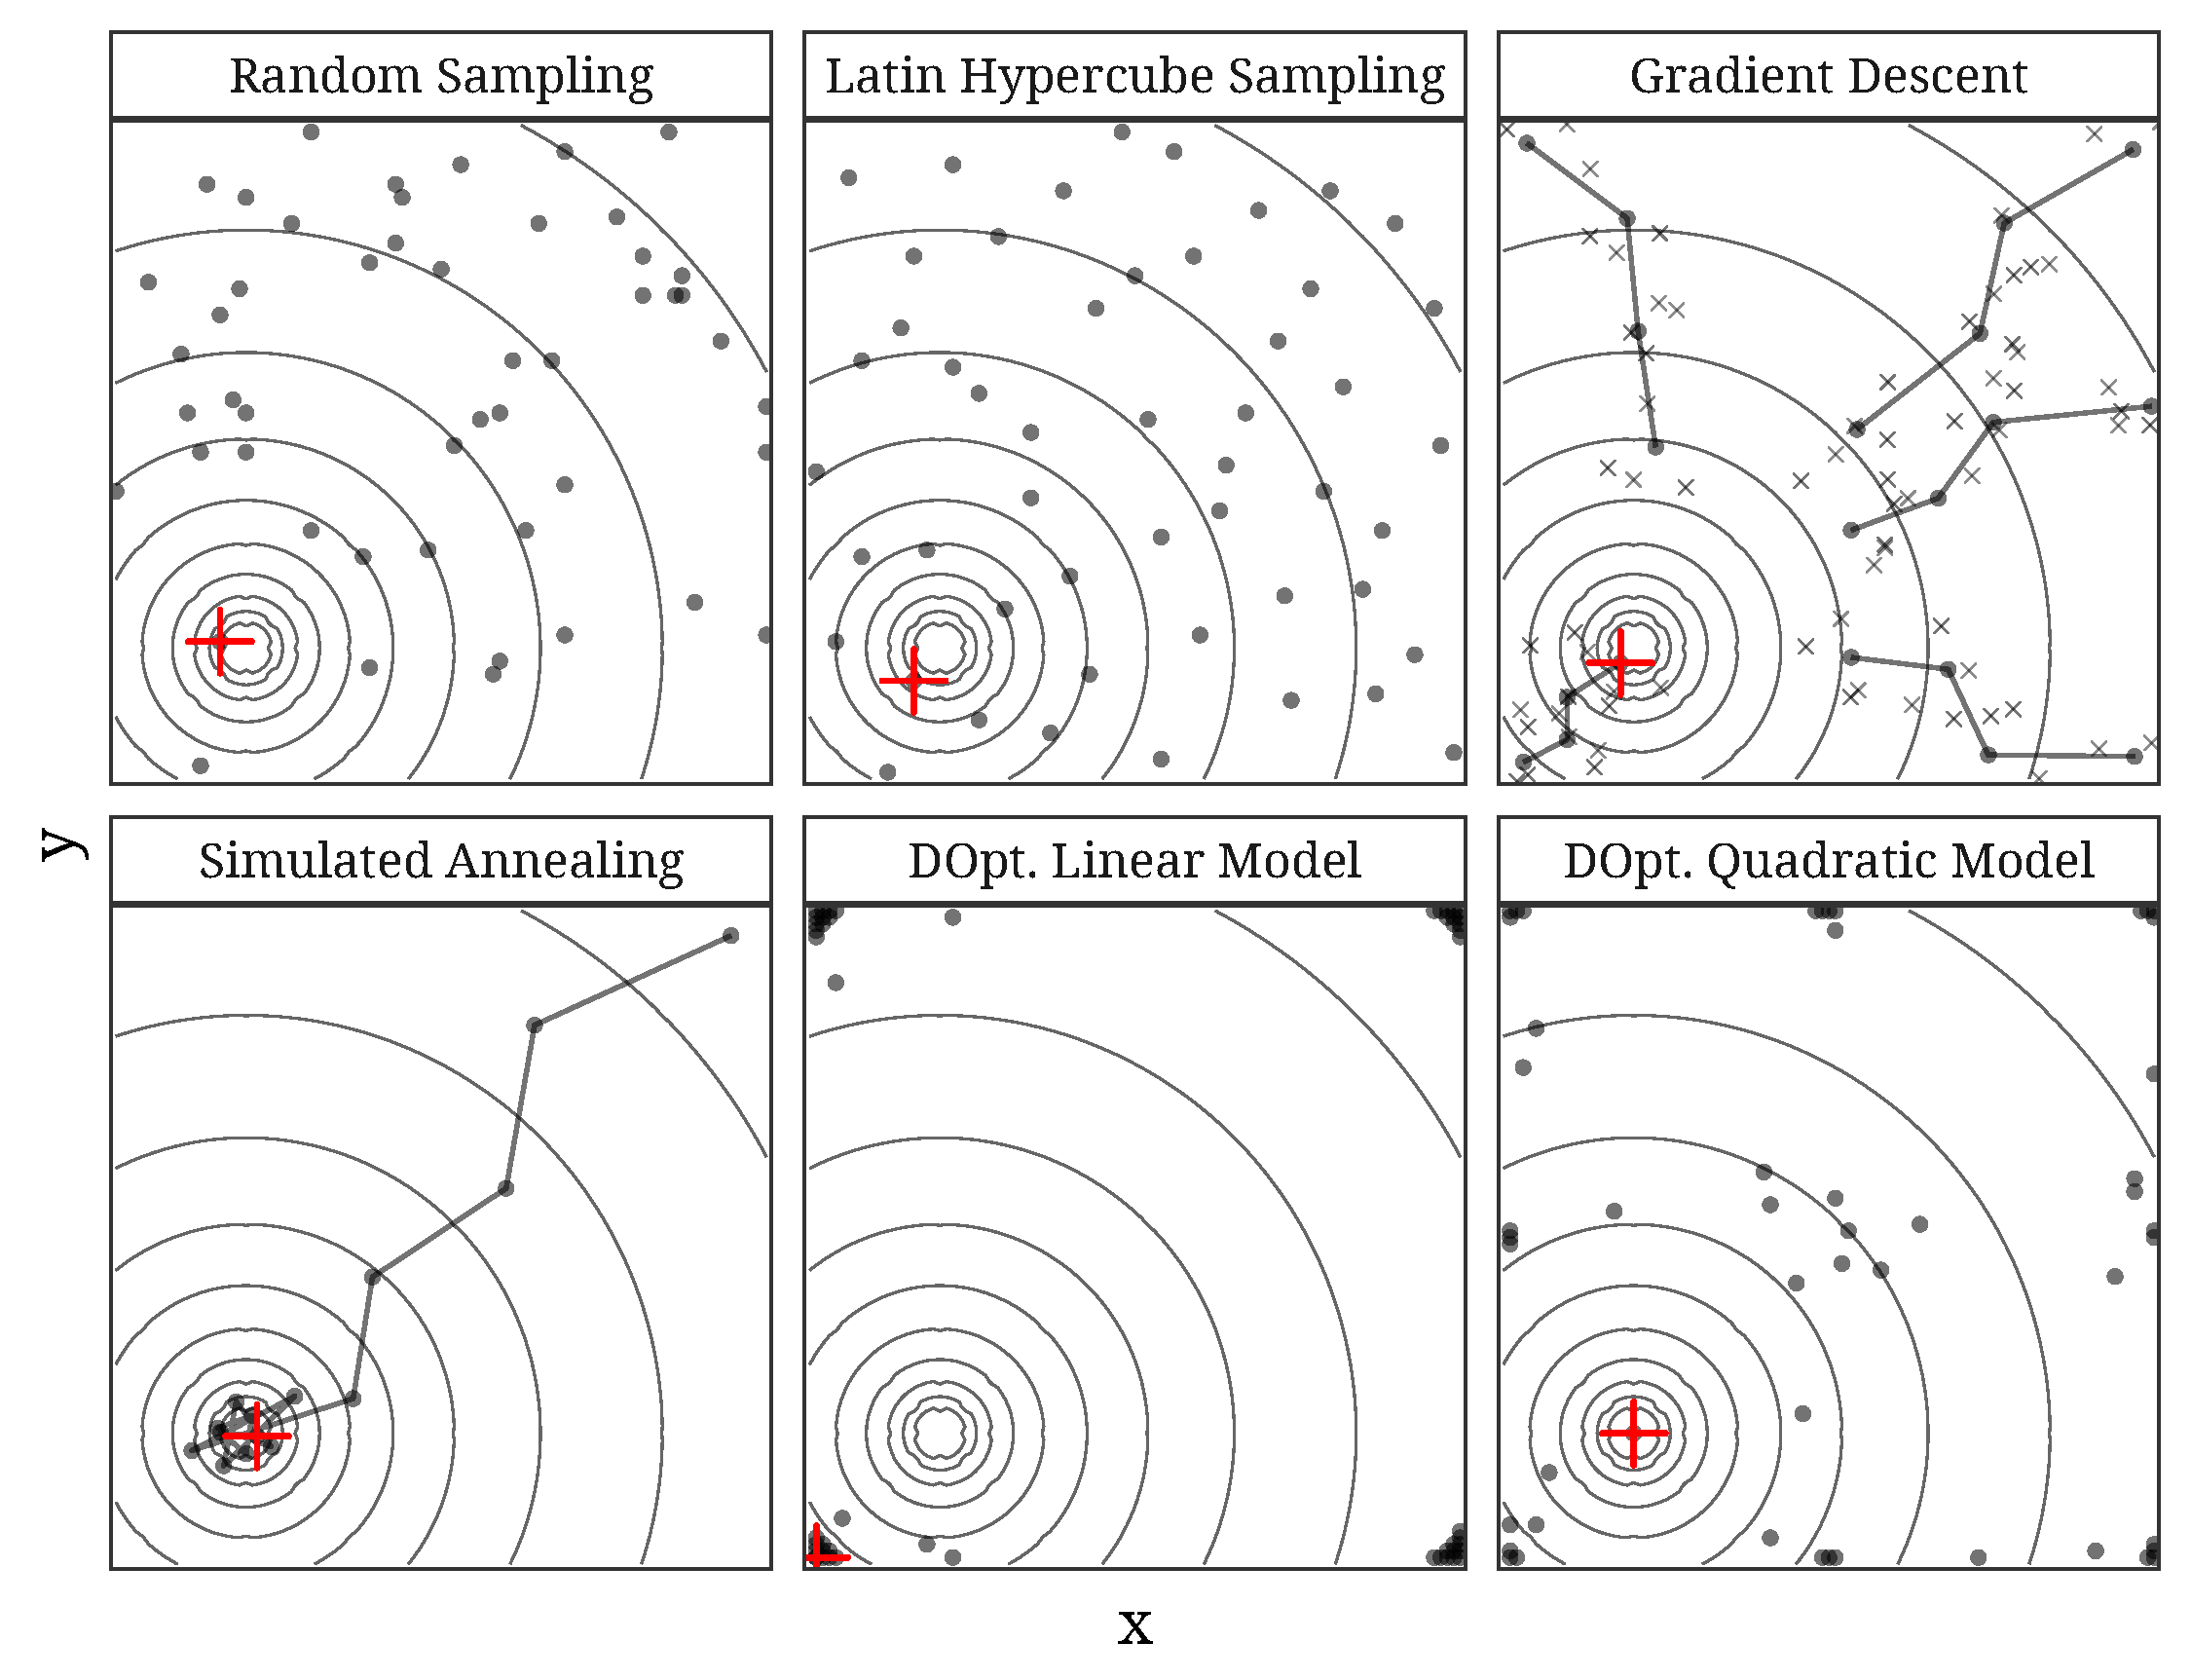
\includegraphics[width=.95\columnwidth]{./img/sampling_comparison.pdf}
\caption{\label{fig:org7a149fd}
Exploration of the search space defined by \(x^2 + y^2\), using a fixed budget of 50 points. The ``\(+\)'' represents the best point found by each strategy}
\end{figure}
\end{center}
\subsection{Autotuning}
\label{sec:org57b7aa7}
John Rice's Algorithm Selection framework~\cite{rice1976algorithm} is the
precursor of autotuners in various problem domains. In 1997, the PHiPAC
system~\cite{bilmes1997optimizing} used code generators and search scripts
to automatically generate high performance code for matrix multiplication. Since
then, systems approached different domains with a variety of strategies.
Dongarra \emph{et al.}~\cite{dongarra1998automatically} introduced the ATLAS
project, that optimizes dense matrix multiplication routines. The
OSKI~\cite{vuduc2005oski} library provides automatically tuned kernels for
sparse matrices. The FFTW~\cite{frigo1998fftw} library provides tuned C
subroutines for computing the Discrete Fourier Transform.
Periscope~\cite{gerndt2010automatic} is a distributed online autotuner for
parallel systems and single-node performance. In an effort to provide a common
representation of multiple parallel programming models, the INSIEME compiler
project~\cite{jordan2012multi} implements abstractions for OpenMP, MPI and
OpenCL, and generates optimized parallel code for heterogeneous multi-core
architectures.

A different approach is to combine generic search algorithms and problem
representation data structures in a single system that enables the
implementation of autotuners for different domains. The
PetaBricks~\cite{ansel2009petabricks} project provides a language,
compiler and autotuner, enabling the definition and selection of multiple
algorithms for the same problem. The ParamILS
framework~\cite{hutter2009paramils} applies stochastic local search
algorithms to algorithm configuration and parameter tuning. The OpenTuner
framework~\cite{ansel2014opentuner} provides ensembles of techniques that
search the same space in parallel, while exploration is managed by a multi-armed
bandit strategy.
\section{Design of Experiments}
\label{sec:org587eea5}
An \emph{experimental design} determines a selection of experiments whose objective
is to identify the relationships between \emph{factors} and \emph{responses}. While
factors and responses can refer to different concrete entities in other domains,
in computer experiments factors can be configuration parameters for algorithms
and compilers, for example, and responses can be the execution time or memory
consumption of a program. Each possible value of a factor is called a \emph{level}.
The \emph{effect} of a factor on the measured response, without its \emph{interactions}
with other factors, is the \emph{main effect} of that factor. Experimental designs
can be constructed with different goals, such as identifying the main effects
or building an analytical model for the response.

In this Section we first present the assumptions of a traditional Design of
Experiments methodology using an example of \emph{2-level screening designs}, which
are an efficient way to identify main effects. We then discuss some techniques
for the construction of efficient designs for factors with arbitrary numbers and
types of levels, and present \emph{D-Optimal} designs, the technique we use in the
approach presented in this paper.
\subsection{Screening \& Plackett-Burman Designs}
\label{sec:org2c64eb2}
Screening designs provide a parsimonious way to identify the main
effects of 2-level factors in the initial stages of studying a problem. While
interactions are not considered at this stage, identifying main effects early
enables focusing on a smaller set of factors on subsequent more detailed
experiments. A specially efficient design construction technique for screening
designs was presented by Plackett and Burman~\cite{plackett1946design} in
1946, and is available in the \texttt{FrF2}
package~\cite{gromping2014frf2} of the \texttt{R}
language~\cite{team2018rlanguage}.

Despite having strong restrictions on the number of factors they support,
Plackett-Burman designs enable the identification of main effects of \(n\) factors
with \(n + 1\) experiments. Factors may have many levels, but Plackett-Burman
designs can only be constructed for 2-level factors. Therefore, before
constructing a Plackett-Burman design we must identify \emph{high} and \emph{low} levels
for each factor.

Assuming a crude linear relationship between factors and the response is
fundamental for running ANOVA tests using a Plackett-Burman design. For the
following example, consider the linear relationship presented in
Equation~\eqref{eq:linear_assumption}, where \(\epsilon\) is the error term,
\(\mathbf{Y}\) is the observed response, \(\mathbf{X} = \left\{1,
x_1,\dots,x_n\right\}\) is the set of \(n\) 2-level factors, and \(\bm{\beta} =
\left\{\beta_0,\dots,\beta_n\right\}\) is the set with the \emph{intercept} \(\beta_0\)
and the corresponding \emph{model coefficients}. ANOVA tests can rigorously compute
the significance of each factor. We can think of that intuitively by noting that
less relevant factors will have corresponding values in \(\bm{\beta}\) close to
zero.

{\normalsize
\begin{align}
\mathbf{Y} = \bm{\beta}\mathbf{X} + \epsilon
%\caption{Linear model assumed in main-effect analysis of screening designs}
\label{eq:linear_assumption}
\end{align}
}

We now present an example to illustrate the screening methodology. Suppose we
wish to minimize a performance metric \(Y\) of a problem with factors
\(x_1,\dots,x_8\) assuming values in \(\left\{-1, -0.8, -0.6, \dots, 0.6, 0.8,
1\right\}\). Each \(y_i \in Y\) is computed using
Equation~\eqref{eq:real_model}, but suppose that, for the purpose of this
example, they are computed by a very expensive black-box procedure. Note that
not all factors are included in the real computation. In this scenario we can
think of the error term \(\epsilon\) as representing not only noise but our
uncertainty regarding the model as well. Higher amplitudes of \(\epsilon\) might
make it harder to justify isolating factors with low significance.

{\normalsize
\begin{align}
\label{eq:real_model}
y_i = & -1.5x_1 + 1.3x_3 + 3.1x_5 + \\
& -1.4x_7 + 1.35x_8^2 + 1.6x_3x_5 + \epsilon \nonumber
\end{align}
%\caption{Real model used to obtain the data on Table\ref{tab:plackett}}
}

To efficiently study this problem we decide to construct a Plackett-Burman
design, which minimizes the experiments needed to identify relevant factors. The
analysis of this design will enable us to decrease the dimension of the problem.
Table~\ref{tab:plackett} presents the Plackett-Burman design we generated.
It contains high and low values, chosen to be \(-1\) and \(1\), for the factors
\(x_1,\dots,x_8\), and the observed response \(\mathbf{Y}\). As is common when
constructing screening designs, we had to add 3 ``dummy'' factors
\(d_1,\dots,d_3\) to complete the 12 columns needed to construct a Plackett-Burman
design for 8 factors.

% latex table generated in R 3.5.1 by xtable 1.8-2 package
% Fri Oct 12 13:46:15 2018
\begin{table}[ht]
\centering
\caption{Randomized Plackett-Burman design for factors $x_1, \dots, x_8$, using 12 experiments and ``dummy'' factors $d_1, \dots, d_3$, and computed response $\mathbf{Y}$}
\label{tab:plackett}
\begingroup\scriptsize
\begin{tabular}{cccccccccccc}
  \toprule
$x_1$ & $x_2$ & $x_3$ & $x_4$ & $x_5$ & $x_6$ & $x_7$ & $x_8$ & $d_1$ & $d_2$ & $d_3$ & $Y$ \\
  \midrule
1 & -1 & 1 & 1 & 1 & -1 & -1 & -1 & 1 & -1 & 1 & 13.74 \\
  -1 & 1 & -1 & 1 & 1 & -1 & 1 & 1 & 1 & -1 & -1 & 10.19 \\
  -1 & 1 & 1 & -1 & 1 & 1 & 1 & -1 & -1 & -1 & 1 & 9.22 \\
  1 & 1 & -1 & 1 & 1 & 1 & -1 & -1 & -1 & 1 & -1 & 7.64 \\
  1 & 1 & 1 & -1 & -1 & -1 & 1 & -1 & 1 & 1 & -1 & 8.63 \\
  -1 & 1 & 1 & 1 & -1 & -1 & -1 & 1 & -1 & 1 & 1 & 11.53 \\
  -1 & -1 & -1 & 1 & -1 & 1 & 1 & -1 & 1 & 1 & 1 & 2.09 \\
  1 & 1 & -1 & -1 & -1 & 1 & -1 & 1 & 1 & -1 & 1 & 9.02 \\
  1 & -1 & -1 & -1 & 1 & -1 & 1 & 1 & -1 & 1 & 1 & 10.68 \\
  1 & -1 & 1 & 1 & -1 & 1 & 1 & 1 & -1 & -1 & -1 & 11.23 \\
  -1 & -1 & -1 & -1 & -1 & -1 & -1 & -1 & -1 & -1 & -1 & 5.33 \\
  -1 & -1 & 1 & -1 & 1 & 1 & -1 & 1 & 1 & 1 & -1 & 14.79 \\
   \bottomrule
\end{tabular}
\endgroup
\end{table}

We use our initial assumption shown in Equation~\eqref{eq:linear_assumption} to
identify the most relevant factors by performing an ANOVA test. The resulting
ANOVA table is shown in Table~\ref{tab:anova_linear}, where the \emph{significance}
of each factor can be interpreted from the F-test and P\((<\text{F})\) values.
Table~\ref{tab:anova_linear} uses ``\(*\)'', as is convention in the \texttt{R}
language, to represent the significance values for each factor.

We see on Table~\ref{tab:anova_linear} that factors
\(\left\{x_3,x_5,x_7,x_8\right\}\) have at least one ``\(*\)'' of significance. For
the purpose of this example, this is sufficient reason to include them in our
linear model for the next step. We decide as well to discard factors
\(\left\{x_2,x_4,x_6\right\}\) in our model for now, due to their low
significance. We see that factor \(x_1\) has a significance mark of ``\(\cdot\)'', but
comparing its F-test and P\((<\text{F})\) values we decide that they are fairly
smaller than the values of factors that had no significance at all, and we keep
this factor.

% latex table generated in R 3.5.1 by xtable 1.8-2 package
% Fri Oct 12 13:58:03 2018
\begin{table}[ht]
\centering
\caption{Shortened ANOVA table for the fit of the naive model, with significance intervals from the \texttt{R} language}
\label{tab:anova_linear}
\begingroup\small
\begin{tabular}{lrrl}
  \toprule
 & F value & Pr$(<\text{F})$ & Signif. \\
  \midrule
$x_1$ & 8.382 & 0.063 & $\cdot$ \\
  $x_2$ & 0.370 & 0.586 &   \\
  $x_3$ & 80.902 & 0.003 & $**$ \\
  $x_4$ & 0.215 & 0.675 &   \\
  $x_5$ & 46.848 & 0.006 & $**$ \\
  $x_6$ & 5.154 & 0.108 &   \\
  $x_7$ & 13.831 & 0.034 & $*$ \\
  $x_8$ & 59.768 & 0.004 & $**$ \\
   \bottomrule
\end{tabular}
\endgroup
\end{table}

Moving forward, we will build a linear model using factors
\(\left\{x_1,x_3,x_5,x_7,x_8\right\}\), fit the model using the values of \(Y\) we
obtained when running our design, and use the coefficients of this fitted model
to predict the levels for each factor that minimize the real response. We can do
that because these factors are numerical, even though only discrete values are
allowed.

We now proceed to the prediction step, where we wish to identify the levels of
factors \(\left\{x_1,x_3,x_5,x_7,x_8\right\}\) that minimize our fitted model,
without running any new experiments. This can be done by, for example, using a
gradient descent algorithm or finding the point where the derivative of the
function given by the linear regression equals to zero.

Table~\ref{tab:linear_prediction_comparison} compares the prediction for
\(Y\) from our linear model with the selected factors
\(\left\{x_1,x_3,x_5,x_7,x_8\right\}\) with the actual global minimum \(Y\) for this
problem. Note that factors \(\left\{x_2,x_4,x_6\right\}\) are included for the
global minimum. This happens here because of the error term \(\epsilon\),
but could also be interpreted as due to model uncertainty.

% latex table generated in R 3.5.1 by xtable 1.8-2 package
% Fri Oct 12 14:06:43 2018
\begin{table}[ht]
\centering
\caption{Comparison of the response $Y$ predicted by the linear model and the true global minimum. Factors used in the model are bolded}
\label{tab:linear_prediction_comparison}
\begingroup\footnotesize
\begin{tabularx}{\columnwidth}{lrlrlrlrrr}
  \toprule
 & $\bm{x_1}$ & $x_2$ & $\bm{x_3}$ & $x_4$ & $\bm{x_5}$ & $x_6$ & $\bm{x_7$} & $\bm{x_8}$ & $Y$ \\
  \midrule
 Lin. & -1.0 & -- & -1.0 & -- & -1.0 & -- & 1.0 & -1.0 & -1.046 \\
  Min. & 1.0 & -0.2 & -1.0 & 0.6 & -1.0 & 0.4 & 0.8 & 0.0 & -9.934 \\
   \bottomrule
\end{tabularx}
\endgroup
\end{table}

Using 12 measurements and a simple linear model, the predicted best
value of \(Y\) was around \(10\times\) larger than the global optimum. Note that the
model predicted the correct levels for \(x_3\) and \(x_5\), and almost predicted
correctly for \(x_7\). The linear model predicted wrong levels for \(x_1\), perhaps
due to this factor's interaction with \(x_3\), and for \(x_8\). Arguably, it would
be impossible to predict the correct level for \(x_8\) using this linear model,
since a quadratic term composes the true formula of \(Y\). As we showed in
Figure~\ref{fig:org7a149fd}, a D-Optimal design using a linear model
could detect the significance of a quadratic term, but the resulting
regression will often predict the wrong minimum point.

We can improve upon this result if we introduce some information about the
problem and use a more flexible design construction technique. Next, we will
discuss the construction of efficient designs using problem-specific formulas
and continue the optimization of our example.
\subsection{D-Optimal Designs}
\label{sec:orgd9e84bc}
The application of Design of Experiments to autotuning problems requires design
construction techniques that support factors of arbitrary types and number of
levels. Autotuning problems typically combine factors such as binary flags,
integer and floating point numerical values, and unordered enumerations of
abstract values. Previously, to construct a Plackett-Burman design for our
example we had to restrict our factors to the extremes of their levels in the
interval \(\left\{-1, -0.8, -0.6,\dots,0.6, 0.8, 1\right\}\), because such designs
only support 2-level factors. We have seen that this restriction makes it
difficult to measure the significance of quadratic terms in the model. We will
now show how to further optimize our example by using \emph{D-Optimal designs}, which
increase the number of levels we can efficiently screen for and enables
detecting the significance of more complex model terms.

To construct a D-Optimal design it is necessary to choose an initial model,
which can be done based on previous experiments or on expert knowledge of the
problem. Once a model is selected, algorithmic construction is performed by
searching for the set of experiments that minimizes \emph{D-Optimality}, a measure of
the \emph{variance} of the \emph{estimators} for the \emph{regression coefficients} associated
with the selected model. This search is usually done by swapping experiments
from the current candidate set with experiments from a pool of possible
experiments, according to certain rules, until some stopping criterion is met.
In the example in this Section, as well as in the approach presented in this
paper, we use Fedorov's algorithm~\cite{fedorov1972theory} for
constructing D-Optimal designs, implemented in \texttt{R} in the \texttt{AlgDesign}
package~\cite{wheeler2014algdesign}.

Going back to our example, suppose that in addition to using our previous
screening results we decide to hire an expert in our problem's domain. The
expert confirms our initial assumptions that the factor \(x_1\) should be included
in our model since it is usually relevant for this kind of problem and has a
strong interaction with factor \(x_3\). She also mentions we should replace
the linear term for \(x_8\) by a quadratic term for this factor.

Using our previous screening and the domain knowledge provided by our expert, we
choose a new performance model and use it to construct a D-Optimal design using
Fedorov's algorithm. Since we need enough degrees of freedom to fit our model,
we construct the design with 12 experiments shown in Table~\ref{tab:d_optimal}.
Note that the design includes \(-1\), \(0\) and \(1\) levels for factor \(x_8\). The design
will sample from different regions of the search space due to the quadratic term,
as was shown in Figure~\ref{fig:org7a149fd}.

% latex table generated in R 3.5.1 by xtable 1.8-2 package
% Fri Oct 12 14:08:40 2018
\begin{table}[ht]
\centering
\caption{D-Optimal design constructed for the factors $\left\{x_1,x_3,x_5,x_7,x_8\right\}$ and computed response $Y$}
\label{tab:d_optimal}
\begingroup\footnotesize
\begin{tabular}{rrrrrr}
  \toprule
$x_1$ & $x_3$ & $x_5$ & $x_7$ & $x_8$ & $Y$ \\
  \midrule
1.0 & -1.0 & -1.0 & -1.0 & -1.0 & -4.881 \\
  1.0 & 1.0 & -1.0 & -1.0 & -1.0 & 1.133 \\
  -1.0 & -1.0 & 1.0 & 1.0 & -1.0 & 4.609 \\
  -1.0 & 1.0 & 1.0 & 1.0 & -1.0 & 3.231 \\
  -1.0 & -1.0 & -1.0 & -1.0 & 0.0 & 0.055 \\
  1.0 & 1.0 & 1.0 & -1.0 & 0.0 & 7.132 \\
  -1.0 & 1.0 & -1.0 & 1.0 & 0.0 & -3.305 \\
  1.0 & -1.0 & 1.0 & 1.0 & 0.0 & -2.187 \\
  -1.0 & -1.0 & 1.0 & -1.0 & 1.0 & 7.854 \\
  -1.0 & 1.0 & 1.0 & -1.0 & 1.0 & 7.336 \\
  1.0 & -1.0 & -1.0 & 1.0 & 1.0 & -8.205 \\
  1.0 & 1.0 & -1.0 & 1.0 & 1.0 & -2.003 \\
   \bottomrule
\end{tabular}
\endgroup
\end{table}

We are now going to fit this model using the results of the experiments in our
D-Optimal design. Table~\ref{tab:correct_fit} shows the model fit table
and compares the estimated and real model coefficients. This example illustrates
that the Design of Experiments approach can achieve close model estimations
using few resources, provided are able to use user input to identify relevant
factors and knowledge about the problem domain to tweak the model.

% latex table generated in R 3.5.1 by xtable 1.8-2 package
% Fri Oct 12 14:08:45 2018
\begin{table}[ht]
\centering
\caption{Correct model fit comparing real and estimated coefficients, with significance intervals from the \texttt{R} language}
\label{tab:correct_fit}
\begingroup\small
\begin{tabular}{lrrrrl}
  \toprule
 & Real & Estimated & t value & Pr$(>|\text{t}|)$ & Signif. \\
  \midrule
Intercept & 0.000 & 0.424 & 2.384 & 0.076 & . \\
  $x_1$ & -1.500 & -1.287 & -11.825 & 0.000 & *** \\
  $x_3$ & 1.300 & 1.357 & 13.218 & 0.000 & *** \\
  $x_5$ & 3.100 & 3.336 & 30.646 & 0.000 & *** \\
  $x_7$ & -1.400 & -1.646 & -15.124 & 0.000 & *** \\
  $x_8$ & 0.000 & 0.111 & 0.886 & 0.426 &   \\
  $x_8^2$ & 1.350 & 0.710 & 3.263 & 0.031 & * \\
  $x_1x_3$ & 1.600 & 1.684 & 15.468 & 0.000 & *** \\
   \bottomrule
\end{tabular}
\endgroup
\end{table}

Table~\ref{tab:prediction_comparisons} compares the global minimum in this
example with the predictions made by our initial linear model from the screening
step and our improved model from this step. Using screening, D-Optimal designs,
and domain knowledge we found an optimization within \(10\%\) of the global
optimum computing \(Y\) only 24 times. We were able to do that by first reducing
the dimension of the problem when we eliminated irrelevant factors in the
screening step. We then constructed a more careful exploration of this new
problem subspace, helped by domain knowledge provided by an expert.

% latex table generated in R 3.5.1 by xtable 1.8-2 package
% Fri Oct 12 14:08:50 2018
\begin{table}[ht]
\centering
\caption{Comparison of the response $Y$ predicted by our models and the true global minimum. Factors used in the models are bolded}
\label{tab:prediction_comparisons}
\begingroup\footnotesize
\begin{tabular}{lrlrlrlrrr}
  \toprule
 & $\bm{x_1}$ & $x_2$ & $\bm{x_3}$ & $x_4$ & $\bm{x_5}$ & $x_6$ & $\bm{x_7$} & $\bm{x_8}$ & $Y$ \\
  \midrule
 Quad. & 1.0 & -- & -1.0 & -- & -1.0 & -- & 1.0 & 0.0 & -9.019 \\
  Lin. & -1.0 & -- & -1.0 & -- & -1.0 & -- & 1.0 & -1.0 & -1.046 \\
  Min. & 1.0 & -0.2 & -1.0 & 0.6 & -1.0 & 0.4 & 0.8 & 0.0 & -9.934 \\
   \bottomrule
\end{tabular}
\endgroup
\end{table}

We are able to explain the performance improvements we obtained in each step of
the process, because we finish steps with a performance model and a performance
prediction. Each factor is included or removed using information obtained in
statistical tests or expert knowledge. If we need to optimize this problem
again, for a different architecture or with larger input, for example, we could
start exploring the search space with a less naive model. We could also continue
the optimization of this problem by further exploring levels of factors
\(\left\{x_2,x_4,x_6\right\}\). The significance of these factors could now be
detectable by ANOVA tests since the other factors are now fixed.

The process of screening for factor significance using ANOVA and fitting a
new model using acquired knowledge is essentially a step in the transparent
Design of Experiments approach we present in the next Section.
\section{Autotuning with Design of Experiments}
\label{sec:org6592dfe}
In this Section we discuss in detail our iterative Design of Experiments
approach to autotuning. At the start of the process it is necessary to define
the factors and levels that compose the search space of the target problem,
select an initial performance model, and generate an experimental design. Then,
as discussed in the previous Section, we identify relevant factors by running an
ANOVA test on the results. This enables selecting and fitting a new performance
model, which is used for predicting levels for each relevant factor. The process
can then restart, generating a new design for the new problem subspace with the
remaining factors. Informed decisions made by the user play a central role in
each iteration, guiding and speeding up the process. Figure
\ref{fig:orgc1111ec} presents an overview of our approach.

The first step of our approach is to define which are the target factors and
which levels of each factor are worth exploring. Then, the user must select an
initial performance model. Compilers typically expose many 2-level factors in
the form of configuration flags. The performance model for a single flag can
only be a linear term, since there are only 2 values to measure. Interactions
between flags can also be considered in an initial model. Numerical factors are
also common, such as block sizes for CUDA programs or loop unrolling amounts.
Deciding which levels to include for these kinds of factors requires a more
careful analysis. For example, if we suspect the performance model has a
quadratic term for a certain factor, we should include at least three of its
levels. The ordering between the levels of other compiler parameters, such as
\texttt{-O(0,1,2,3)}, is not obviously translated to a numerical ordering.
Factors like these are named \emph{categorical}, and must be treated differently when
constructing designs and analyzing the results.

\begin{center}
\begin{figure}[htbp]
\centering
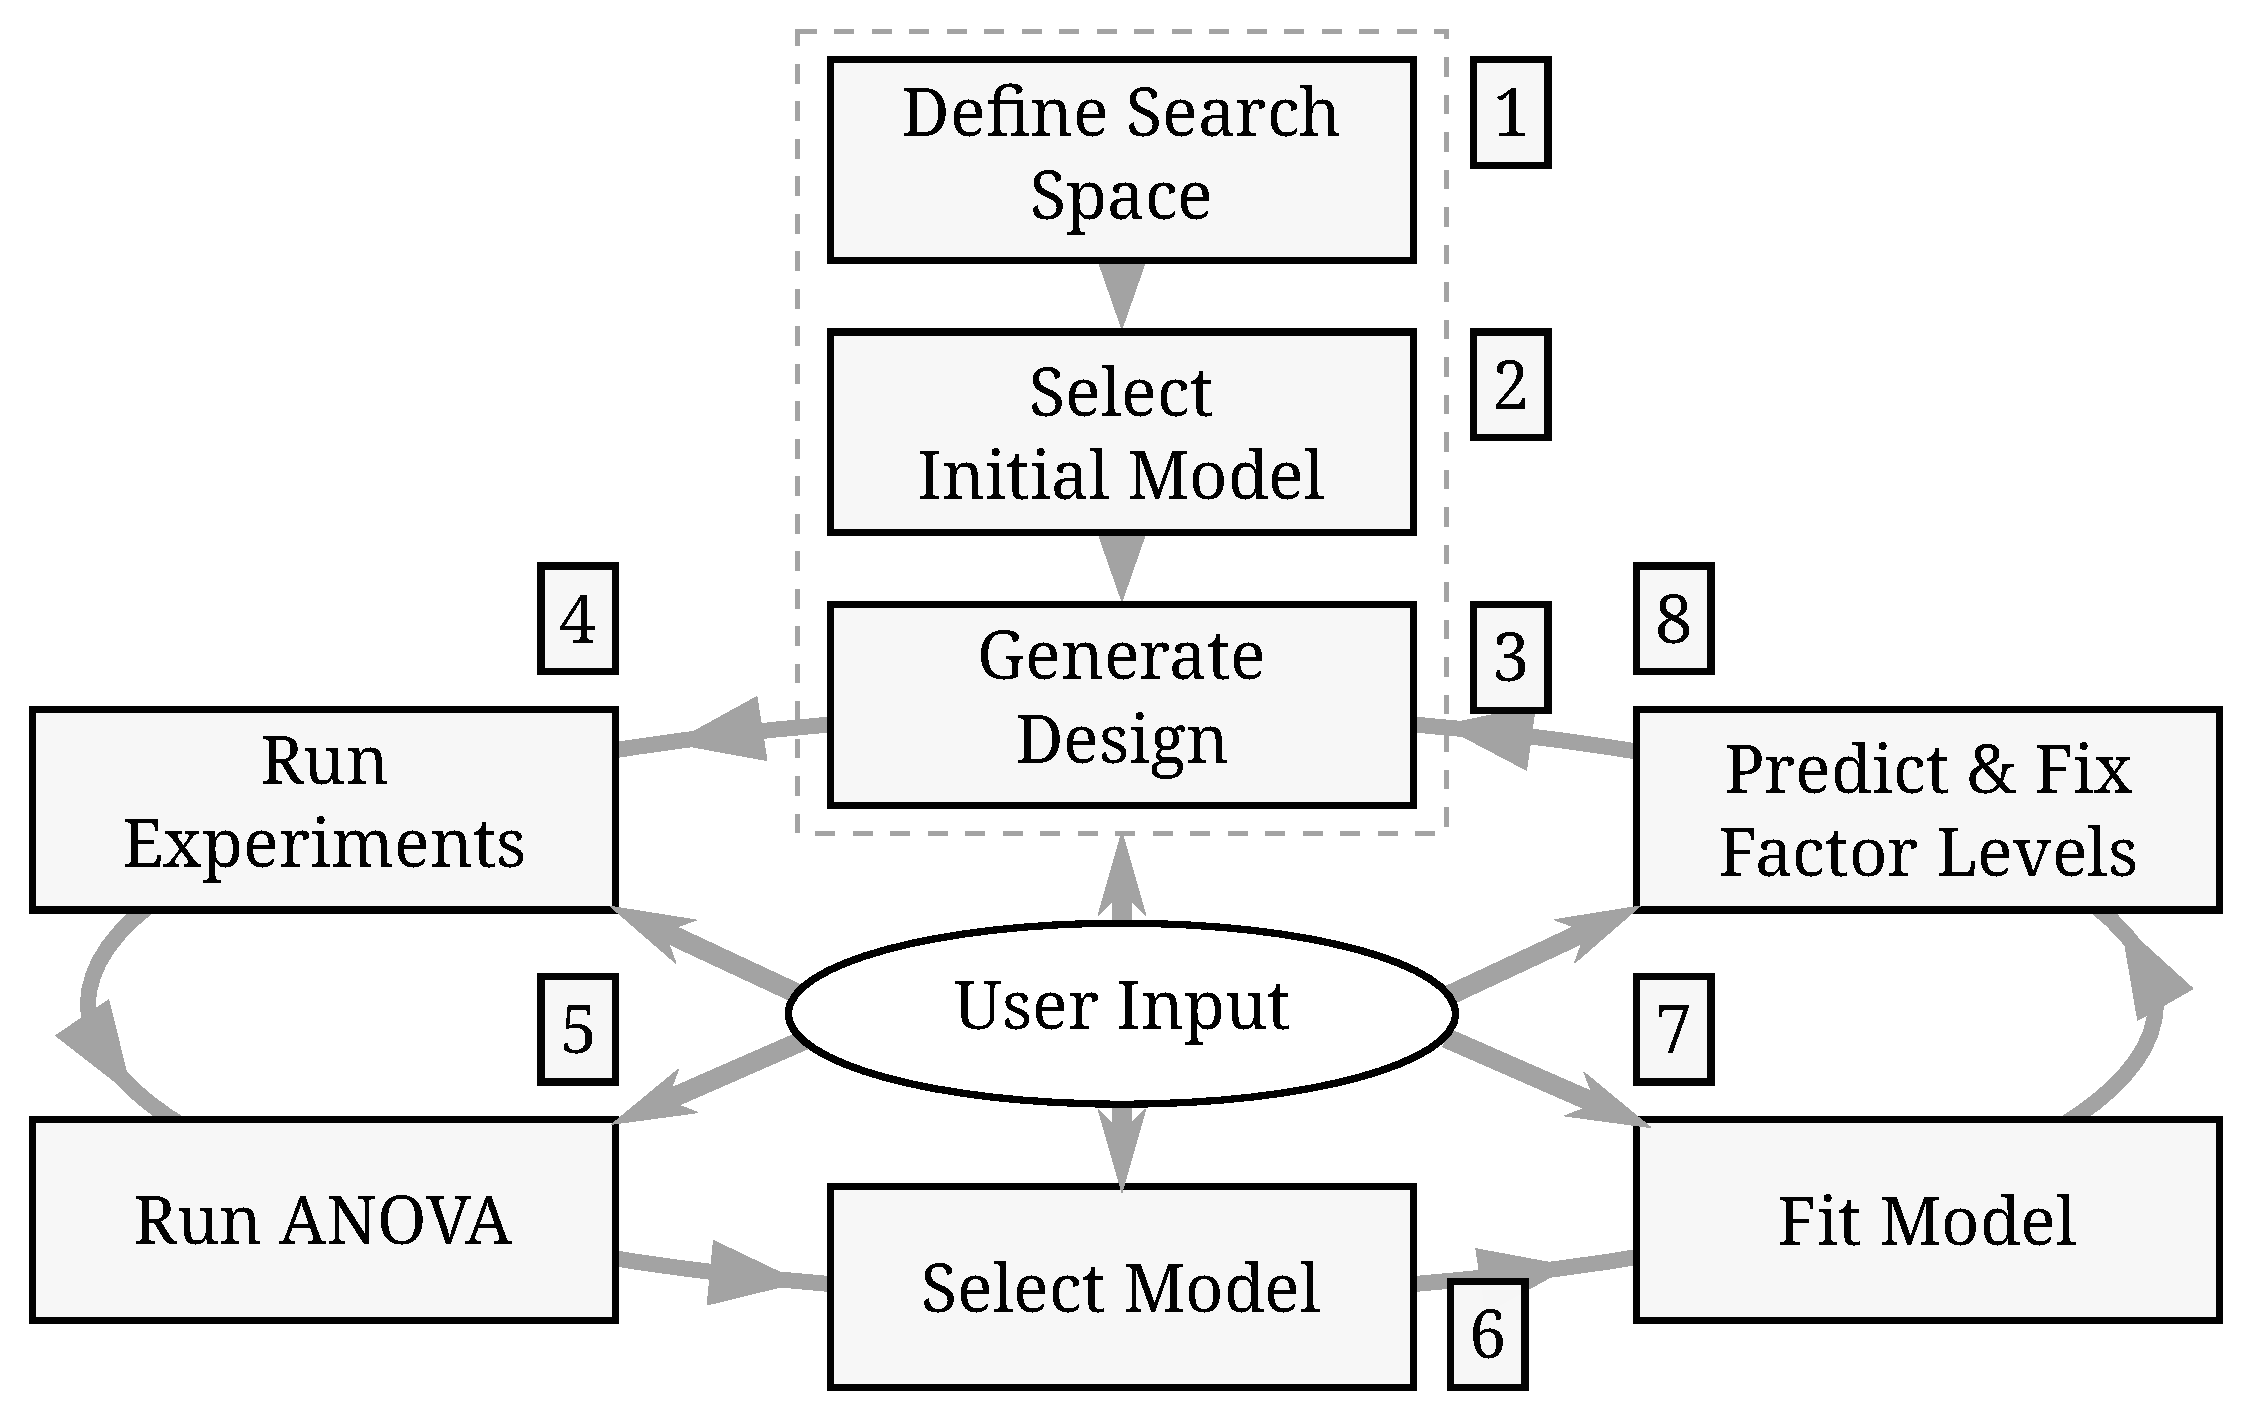
\includegraphics[width=.95\columnwidth]{./img/doe_anova_strategy.pdf}
\caption{\label{fig:orgc1111ec}
Overview of the Design of Experiments approach to autotuning proposed in this paper}
\end{figure}
\end{center}

We decided to use D-Optimal designs because their construction techniques enable
mixing categorical and numerical factors in the same screening design, while
biasing sampling according to a performance model. This enables the autotuner to
exploit global search space structures if we use the right model. When
constructing a D-Optimal design the user can require that specific points in the
search space are included, or that others are not. Algorithms for constructing
D-Optimal designs are capable of adapting to these requirements by optimizing a
starting design. Before settling on D-Optimal designs, we explored other design
construction techniques such as the
Plackett-Burman~\cite{plackett1946design} screening designs shown in the
previous Section, the \emph{contractive replacement} technique of
Addelman-Kempthorne~\cite{addelman1961some} and the \emph{direct generation}
algorithm by Grömping and Fontana~\cite{ulrike2018algorithm}. These
techniques have strong requirements on design size and level mixing, so we opted
for a more flexible technique that would enable exploring a more comprehensive
class of autotuning problems.

After the design is constructed we run each selected experiment. This step can
be done in parallel since experiments are independent. Runtime failures are
common in this step due to problems such as incorrect output. The user can
decide whether to construct a new design using the successfully completed
experiments or to continue to the analysis step if enough experiments succeed.

The next four steps of an iteration, shown in Figure \ref{fig:orgc1111ec},
were discussed in detail in the previous Section. User input is fundamental to
the success of these steps. After running the ANOVA test, the user should apply
domain knowledge to analyze the ANOVA table and determine which factors are
relevant. Certain factors might not appear relevant but the user might still
want to include them in the model to explore more of its levels, for example.
Selecting the model after the ANOVA test also benefits from domain knowledge.
The impact of the number of threads used by a parallel program on its
performance is usually modeled using a quadratic term, for example.

A central assumption of ANOVA is the \emph{homoscedasticity} of the response, which
can be interpreted as requiring the observed error on measurements to be
independent of factor levels and of the number of measurements. Fortunately, up
to a point, there are statistical tests and corrections for lack of
homoscedasticity. Our approach uses the homoscedasticity check and correction by
power transformations from the \texttt{car} package~\cite{fox2011car} of the \texttt{R}
language before every ANOVA step.

The prediction step uses the fitted model to find factor levels that minimize
the response. The choice of the method to find these levels depends on factor
types and model and search space complexity. If factors have discrete levels,
neighborhood exploration might be needed to find valid levels that minimize the
response around the predicted levels. Validity constraints might put predicted
levels on an undefined or invalid region on the search space. This presents a
harder challenge, where the borders of valid regions would have to be explored.

The last step of an iteration is fixing factor levels to those predicted to have
best performance. The user can also decide the level of trust that will be
placed on the model and ANOVA at this step by allowing other levels. This step
performs a reduction on the dimension of the problem by eliminating factors and
decreasing the size of the search space. If we identify relevant parameters
correctly, we will have restricted further search to better regions of the
search space. In the next Section we present the performance of our approach in
scenarios that differ on search space size, availability and complexity.
\section{Performance Evaluation}
\label{sec:orge528b74}
In this Section we present performance evaluations of our approach in two
scenarios.
\subsection{GPU Laplacian Kernel}
\label{sec:org0fd1952}
We first evaluated the performance of our approach in a Laplacian Kernel
implemented using BOAST~\cite{videau2017boast} and targeting the Nvidia
K40c GPU. The objective was to minimize the \emph{time to compute each pixel} by
finding the best level combination for the factors listed in Table
\ref{tab:org3f00f67}. Considering only factors and levels, the size of the
search space is \(1.9\times10^5\) but removing points that fail at runtime yields
a search space of size \(2.3\times10^4\). The complete search space took 154 hours
to be evaluated on \emph{Debian Jessie}, using an \emph{Intel Xeon E5-2630v2} CPU,
\texttt{gcc} version \texttt{4.8.3} and Nvidia driver version \texttt{340.32}.

\begin{table}[ht]
\caption{\label{tab:org3f00f67}
Parameters of the Laplacian Kernel}
\centering
\footnotesize
\begin{tabular}{ll}
\toprule
Factor & Levels\\
\midrule
\texttt{vector\_length} & \(2^0,\dots,2^4\)\\
\texttt{load\_overlap} & \textit{true}, \textit{false}\\
\texttt{temporary\_size} & \(2,4\)\\
\texttt{elements\_number} & \(1,\dots,24\)\\
\texttt{y\_component\_number} & \(1,\dots,6\)\\
\texttt{threads\_number} & \(2^5,\dots,2^{10}\)\\
\texttt{lws\_y} & \(2^0,\dots,2^{10}\)\\
\bottomrule
\end{tabular}
\end{table}

We applied domain knowledge to construct the initial performance model shown in
Equation~\eqref{eq:gpu_laplacian_performance_model}. This performance model
was used by the Iterative Linear Model (LM) algorithm and by our D-Optimal
Design approach (DLMT). The LM algorithm is identical to our approach, described
Section~\ref{sec:org6592dfe}, except for the design
generation step, where it uses a fixed-size random sample of the search space
instead of generating designs. We compared the performance of our approach with
the algorithms listed in Table~\ref{tab:orgb51795f}, using a
budget of \emph{at most} 125 measurements and 1000 repetitions.

{\scriptsize
\begin{align}
%\caption{Initial performance model used by LM and DLMT}
\label{eq:gpu_laplacian_performance_model}
\texttt{time\_per\_pixel} \sim & \; \texttt{y\_component\_number} + 1 / \texttt{y\_component\_number} \; + \nonumber \\
& \; \texttt{vector\_length} + \texttt{lws\_y} + 1 / \texttt{lws\_y} \; + \nonumber \\
& \; \texttt{load\_overlap} + \texttt{temporary\_size} \; + \\
& \; \texttt{elements\_number} + 1 / \texttt{elements\_number} \; + \nonumber \\
& \; \texttt{threads\_number} + 1 /\texttt{threads\_number} \nonumber
\end{align}
}

\begin{table}[ht]
\caption{\label{tab:orgb51795f}
Search algorithms compared in the GPU Laplacian Kernel}
\centering
\footnotesize
\begin{tabular}{ll}
\toprule
 & Algorithm\\
\midrule
RS & Random Sampling\\
LHS & Latin Hyper Square Sampling\\
GS & Greedy Search\\
GSR & Greedy Search w/ Restart\\
GA & Genetic Algorithm\\
LM & Iterative Linear Model\\
DLMT & D-Optimal Designs\\
\bottomrule
\end{tabular}
\end{table}

Table~\ref{tab:gpu_laplacian_compare_budget} shows the mean, minimum and
maximum \emph{slowdowns}, in comparison to the global minimum, for each algorithm. It
also shows the mean and maximum budget used by each algorithm.
Figure~\ref{fig:org8226696} presents histograms for the
slowdowns found by each of the 1000 repetitions. Arrows point the maximum
slowdown found by each algorithm.

% latex table generated in R 3.5.1 by xtable 1.8-2 package
% Fri Oct 12 15:27:06 2018
\begin{table}[ht]
\centering
\caption{Slowdown and budget used by 7 optimization methods on the Laplacian Kernel, using a budget of 125 points with 1000 repetitions}
\label{tab:gpu_laplacian_compare_budget}
\begingroup\footnotesize
\begin{tabular}{lrrrrr}
  \toprule
 & Mean & Min. & Max. & Mean Budget & Max. Budget \\
  \midrule
RS & 1.10 & 1.00 & 1.39 & 120.00 & 120.00 \\
  LHS & 1.17 & 1.00 & 1.52 & 98.92 & 125.00 \\
  GS & 6.46 & 1.00 & 124.76 & 22.17 & 106.00 \\
  GSR & 1.23 & 1.00 & 3.16 & 120.00 & 120.00 \\
  GA & 1.12 & 1.00 & 1.65 & 120.00 & 120.00 \\
  LM & 1.02 & 1.01 & 3.77 & 119.00 & 119.00 \\
   \rowcolor{red!25}DLMT & 1.01 & 1.01 & 1.01 & 54.84 & 56.00 \\
   \bottomrule
\end{tabular}
\endgroup
\end{table}

All algorithms performed well in this kernel, with only Greedy Search (GS)
not being able to find slowdowns smaller than 4\(\times\) in some runs. As
expected, other search algorithms had results similar to Random Sampling (RS).
The LM algorithm was able to find the global minimum on most runs, but some runs
found slowdowns of almost \(4\times\). Our approach was able to find the global
minimum in all of the 1000 runs while using \emph{at most} less than half of the
allotted budget.

\begin{center}
\begin{figure}[ht]
\centering
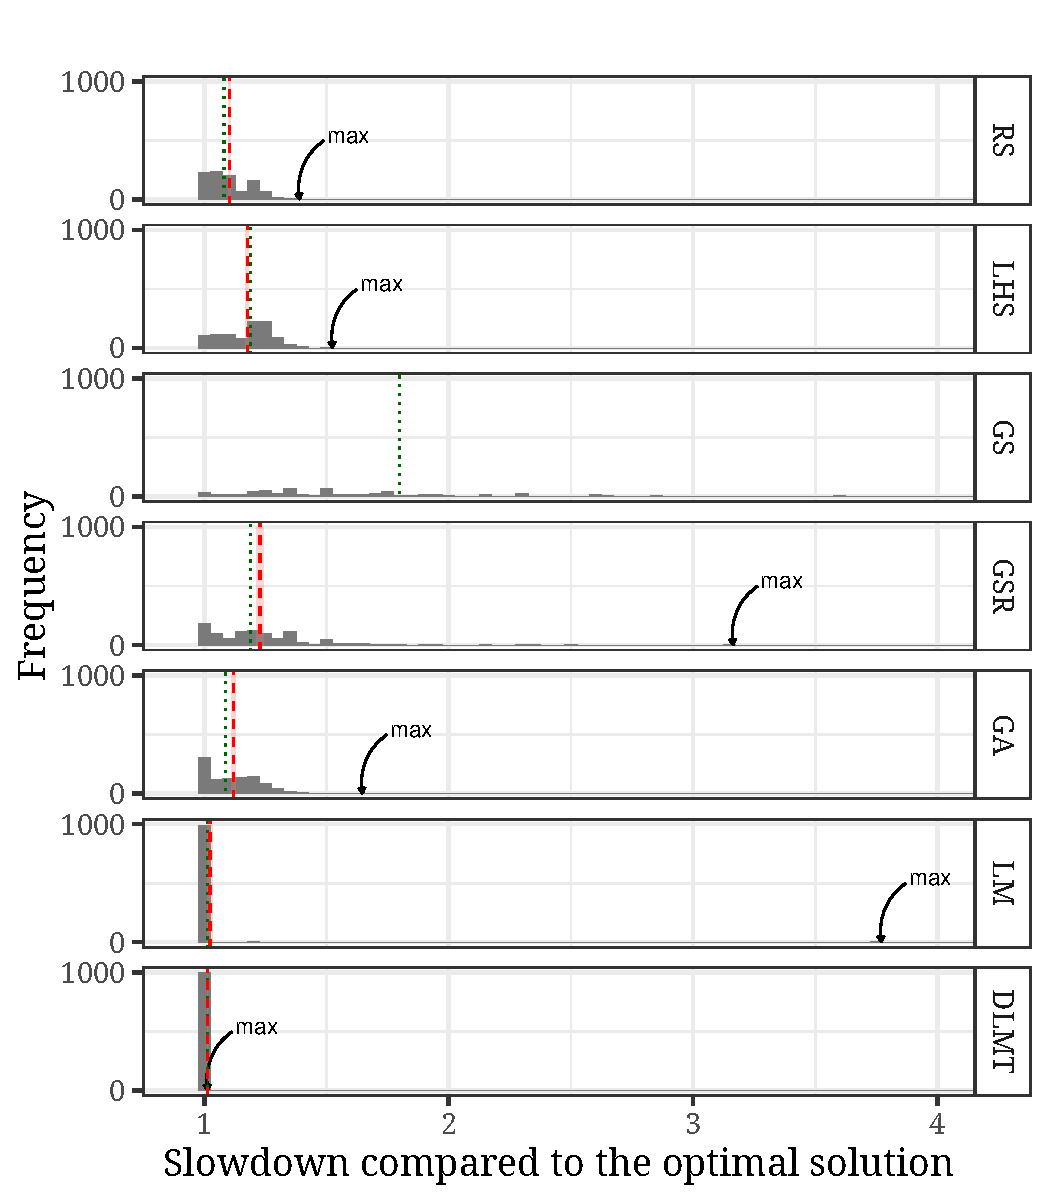
\includegraphics[width=.9\columnwidth]{./img/comparison_histogram.pdf}
\caption{\label{fig:org8226696}
Histograms of 7 optimization methods on the Laplacian Kernel, using a budget of 125 points with 1000 repetitions}
\end{figure}
\end{center}

This kernel provides ideal conditions for using our approach, where the
performance model is approximately known and the complete valid search space is
small enough to be stored and used for prediction. The global minimum also
appears to not be isolated in a region of points with bad performance, since our
approach was able to exploit search space geometry. Next we will analyze the
performance of our approach in a larger and more comprehensive scenario.
\subsection{SPAPT Benchmark}
\label{sec:orga17ad47}
The SPAPT~\cite{balaprakash2012spapt} benchmark provides parametrized
kernels from different High Performance Computing domains. The kernels, shown in
\todo{valid size}Table~\ref{tab:org97d1f8a}, are implemented using the code annotation and
transformation tools provided by Orio~\cite{hartono2009annotation}. Search
space sizes are overall larger than in the Laplacian Kernel example. Kernel factors
are either integers in a range, such as loop unrolling and register tiling amounts,
or binary flags that control parallelization and vectorization, for example.

We used the Random Sampling (RS) implementation available in Orio and
implemented our approach (DLMT) in the system.

\todo{!}After the model is selected and fitted, prediction results will depend
on the size of the data set available. If it is feasible to compute the fitted
model on all possible factor combinations, we can be sure that the global
optimum has a chance of being found. If the search space is too large to be
generated, we have to adapt this step and run the prediction on a sample.

\begin{table}[ht]
\caption{\label{tab:org97d1f8a}
Set of kernels we used from the SPAPT benchmark}
\centering
\scriptsize
\begin{tabular}{llll}
\toprule
Kernel & Operation & Factors & Size\\
\midrule
\texttt{atax} & Matrix transp. \& vector mult. & 18 & \(2.6 \times 10^{16}\)\\
\texttt{dgemv3} & Scalar, vector \& matrix mult. & 49 & \(3.8 \times 10^{36}\)\\
\texttt{gemver} & Vector mult. \& matrix add. & 24 & \(2.6 \times 10^{22}\)\\
\texttt{gesummv} & Scalar, vector, \& matrix mult. & 11 & \(5.3 \times 10^{9}\)\\
\texttt{hessian} & Hessian computation & 9 & \(3.7 \times 10^{7}\)\\
\texttt{mm} & Matrix multiplication & 13 & \(1.2 \times 10^{12}\)\\
\texttt{mvt} & Matrix vector product \& transp. & 12 & \(1.1 \times 10^{9}\)\\
\texttt{tensor} & Tensor matrix mult. & 20 & \(1.2 \times 10^{19}\)\\
\texttt{trmm} & Triangular matrix operations & 25 & \(3.7 \times 10^{23}\)\\
\texttt{bicg} & Subkernel of BiCGStab & 13 & \(3.2 \times 10^{11}\)\\
\texttt{lu} & LU decomposition & 14 & \(9.6 \times 10^{12}\)\\
\texttt{adi} & Matrix sub., mult., \& div. & 20 & \(6.0 \times 10^{15}\)\\
\texttt{jacobi} & 1-D Jacobi computation & 11 & \(5.3 \times 10^{9}\)\\
\texttt{seidel} & Matrix factorization & 15 & \(1.3 \times 10^{14}\)\\
\texttt{stencil3d} & 3-D stencil computation & 29 & \(9.7 \times 10^{27}\)\\
\texttt{correlation} & Correlation computation & 21 & \(4.5 \times 10^{17}\)\\
\bottomrule
\end{tabular}
\end{table}

\begin{center}
\begin{figure*}[p]
\centering
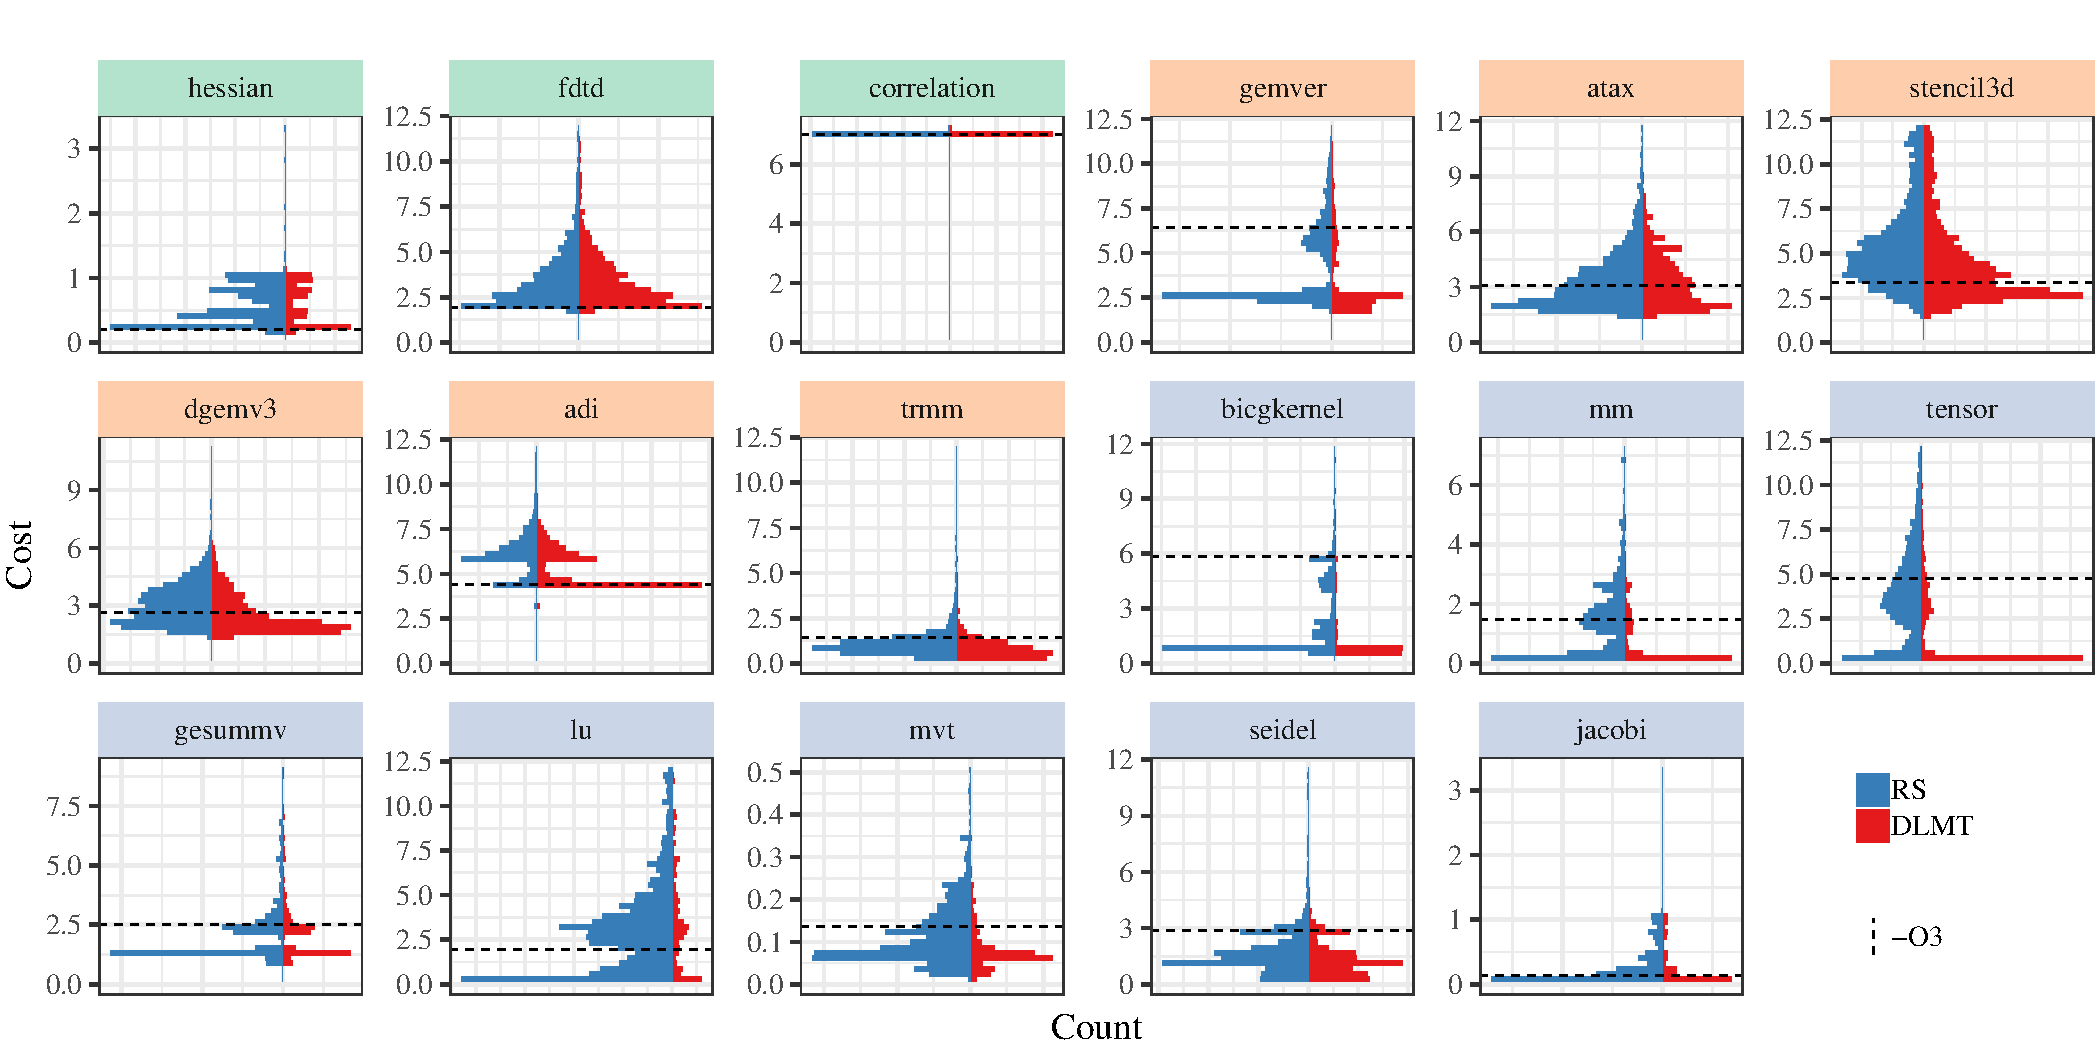
\includegraphics[width=\textwidth]{./img/split_histograms.pdf}
\caption{\label{fig:org6625fc8}
Histograms of explored search spaces}
\end{figure*}
\end{center}

\begin{center}
\begin{figure*}[p]
\centering
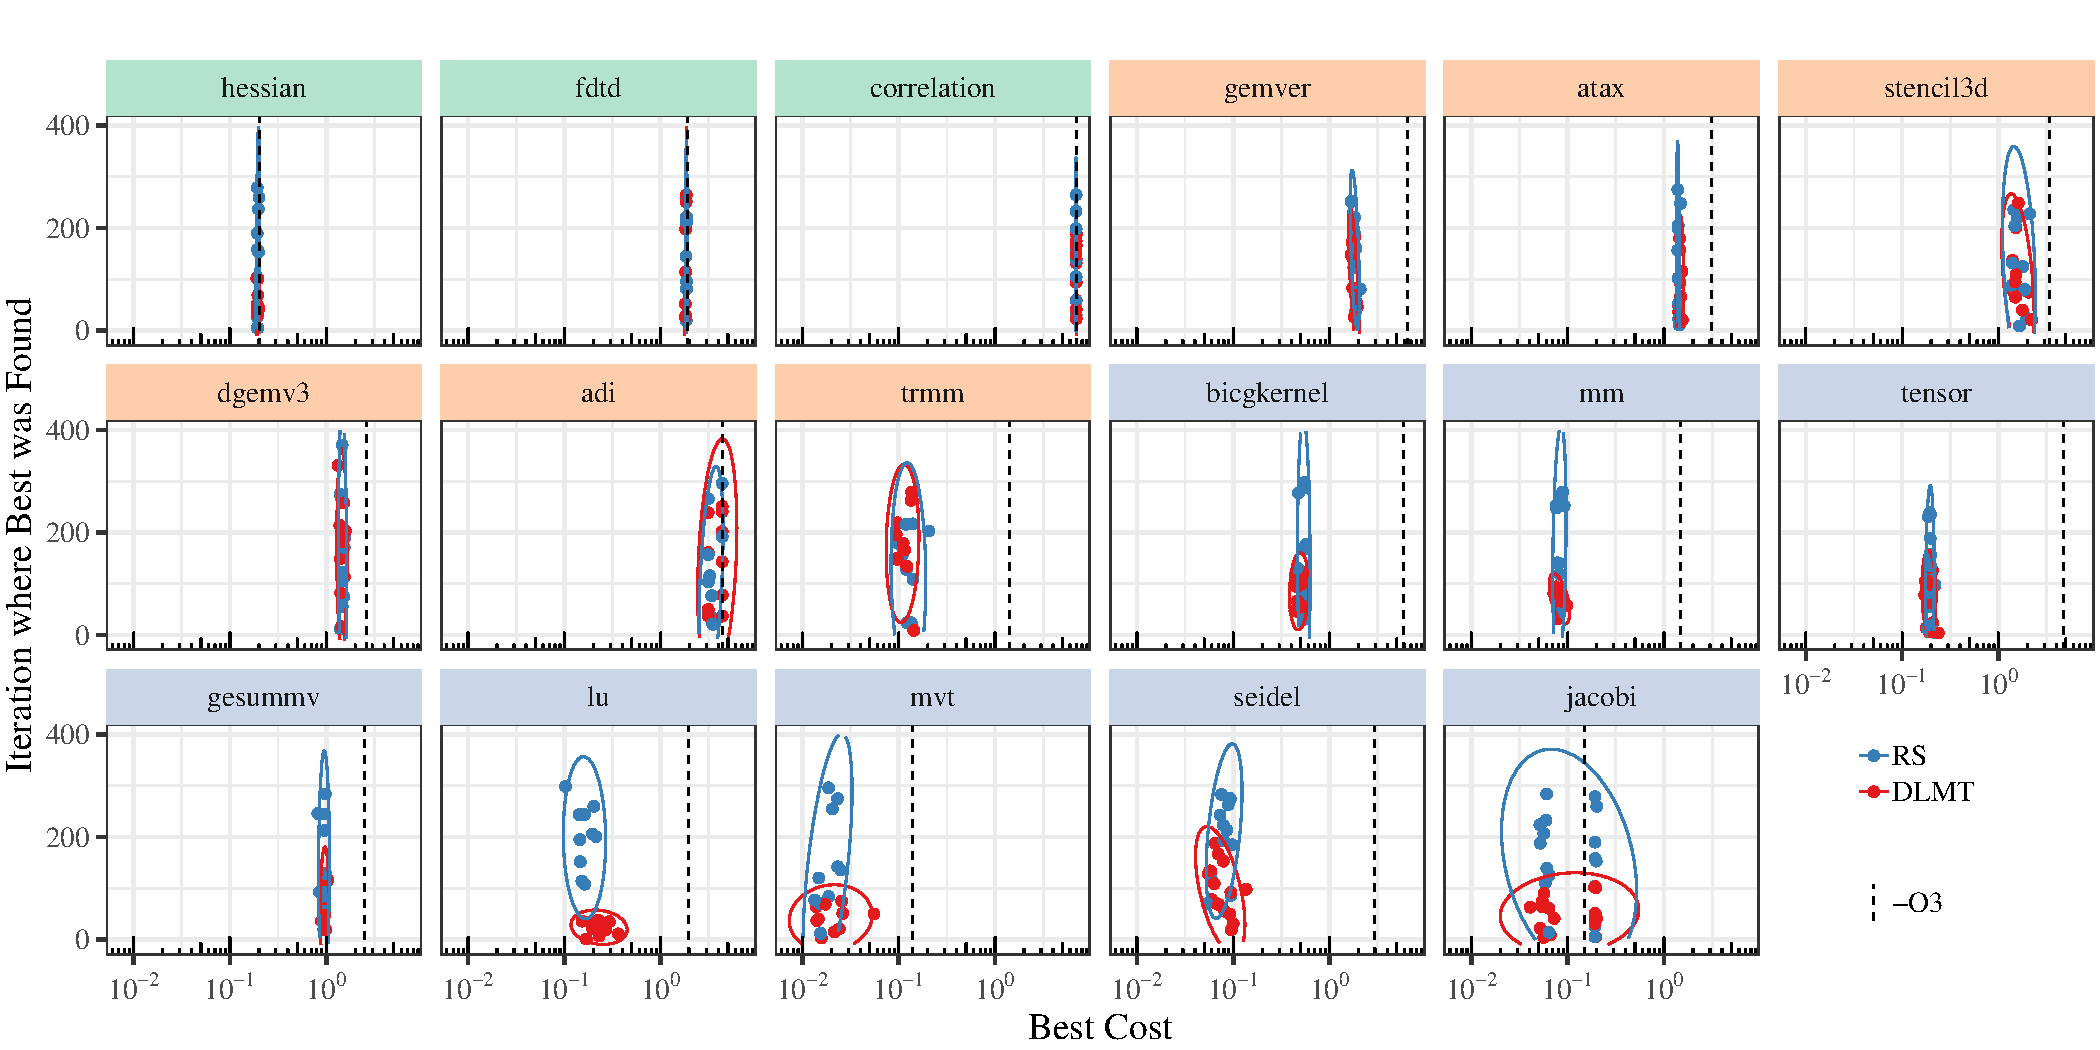
\includegraphics[width=\textwidth]{./img/iteration_best_comparison.pdf}
\caption{\label{fig:org6b6fbcf}
Cost of best point found on each run against the iteration where it was found}
\end{figure*}
\end{center}
\section{Conclusion}
\label{sec:org6ee9368}
\section*{Acknowledgment}
\label{sec:org52ad49f}
\bibliographystyle{IEEEtran}
\bibliography{references}
\end{document}
